\documentclass[class=report, crop=false, 12pt,a4paper]{standalone}
\usepackage{enumitem}
\usepackage{multicol}
\usepackage{graphicx}
\usepackage{float}
\usepackage{amsmath}
\usepackage{amssymb}
\usepackage{mathtools}
\usepackage{siunitx}
\usepackage{commath}
\usepackage{array}
\usepackage{natbib}
\usepackage[a4paper,width=150mm,top=25mm,bottom=25mm]{geometry}
\setlength{\parindent}{0pt}
\begin{document}
\begin{center}
  09/10/2020
\end{center}
\section{Internal Forces and Diagrams}
\subsection{Bending Moment}
The \textbf{bending moment}  is by far the most relevant of the internal forces, since it produces the largest levels of deformations and stress into the beam.
Therefore, it is essential to be able to determine the distribution of the bending moment along the members, in order to assess the mechanical and functional safety of the structure.
\subsection{Diagrams and Determination of Internal Forces}
To determine the internal forces of a body, and draw the relevant diagrams, the following steps are followed:
\subsubsection{Step 1}
Apply to the body the force and moment equilibrium equations to find support reactions (it is possible only if the system is statically determinate)
\subsubsection{Step 2}
Imagine to cut the beam at a section at a distance $x$ from the beam extreme. Balance the forces and moments of the rigid body by applying the required forces and moment at the cut section
\begin{itemize}[noitemsep]
  \item The \textbf{Shear Force} on any given section of a structural member is the algebraic sum of the forces to \textbf{one side only} of the section considered.
  \item The \textbf{Bending Moment} on any given section of a structural member is the algebraic sum of the moments of all the forces to \textbf{one side only} of the section, about the section
  \item The maximum value of bending moment occurs at the point where the Shear Force is zero
\end{itemize}
\subsubsection{Example: Cantilever beam having combined concentrated and distributive loads}
\begin{figure}[H]
  \centering
  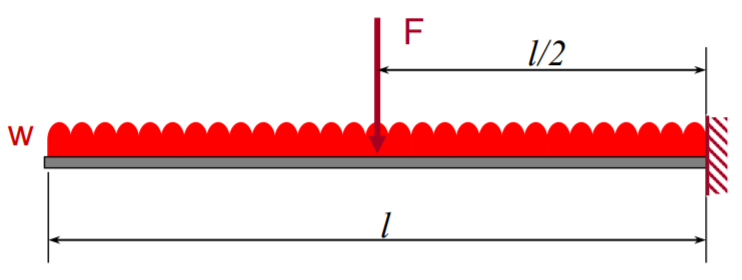
\includegraphics[width = 0.7 \textwidth]{../img/cantileverbeam.PNG}
\end{figure}
\subsubsection{Determination of Support Reactions:}
\begin{figure}[H]
  \centering
  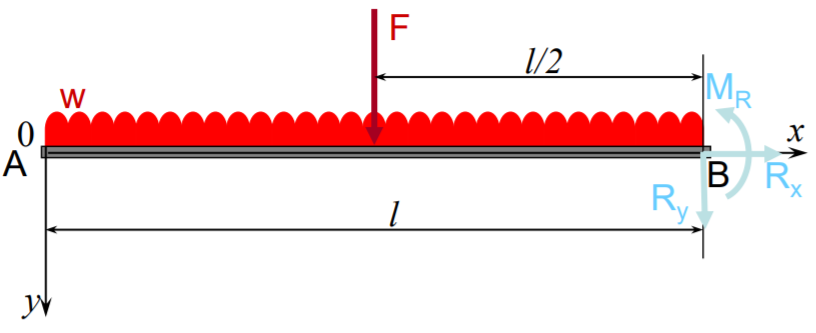
\includegraphics[width = 0.75 \textwidth]{../img/supportreactions.PNG}
\end{figure}
\begin{center}
  $\vec{R_B} = \left[ \begin{array}{ccc} R_x \\ R_y \\ M \end{array}\right]$
\end{center}
\begin{gather}
  \sum F_x: R_x = 0 \\
  \sum F_y: R_y + F + wl = 0 \\
  R_y = -(F+wl) \\
  \sum M: M - F\frac{l}{2} - wl\frac{l}{2} = 0 \\
  M = F\frac{l}{2} + wl\frac{l}{2} = \frac{Fl+wl^2}{2}
\end{gather}
\subsubsection{Determination of internal forces (from $x=0$ to $x=\frac{l}{2}$)}
\begin{figure}[H]
  \centering
  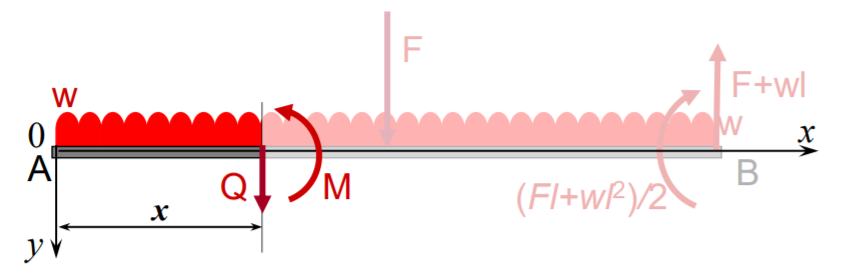
\includegraphics[width = 0.8 \textwidth]{../img/determinationofforces1.PNG}
\end{figure}
\begin{gather}
  \sum F_y: Q + wx = 0 \\
  Q = -wx
\end{gather}
$Q$ varies linearly: it is zero at $x=0$ and is $\frac{-wl}{2}$ at $x=\frac{l}{2}$.
\begin{gather}
  \sum M: M_x + wx\frac{x}{2} = 0 \\
  M_x = \frac{-wx^2}{2}
\end{gather}
$M$ varies parabolically: it is zero at $x=0$ and $\frac{-wl^2}{8}$ at $x=\frac{l}{2}$.
\subsubsection{Determination of internal forces (from $x=\frac{l}{2}$ to $x=l$)}
\begin{figure}[H]
  \centering
  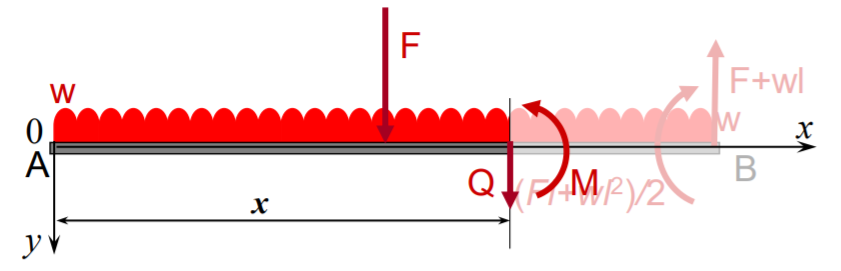
\includegraphics[width = 0.8 \textwidth]{../img/determinationofforces2.PNG}
\end{figure}
\begin{gather}
  \sum F_y: Q + wx + F = 0 \\
  Q = -wx -F
\end{gather}
$Q$ varies linearly between $x=\frac{l}{2}$ (where it is $-(\frac{wl}{2}+F)$) and $x=l$ (where it is $-(F+wl)$)
\begin{gather}
  \sum M: M_x + wx\frac{x}{2} + F(x-\frac{l}{2})= 0 \\
  M_x = \frac{-wx^2}{2} - F(x-\frac{l}{2})
\end{gather}
At $x=\frac{l}{2}$, $M$ distribution changes into a parabola with a steeper slope
\subsubsection{Diagram of Internal Forces}
\begin{figure}[H]
  \centering
  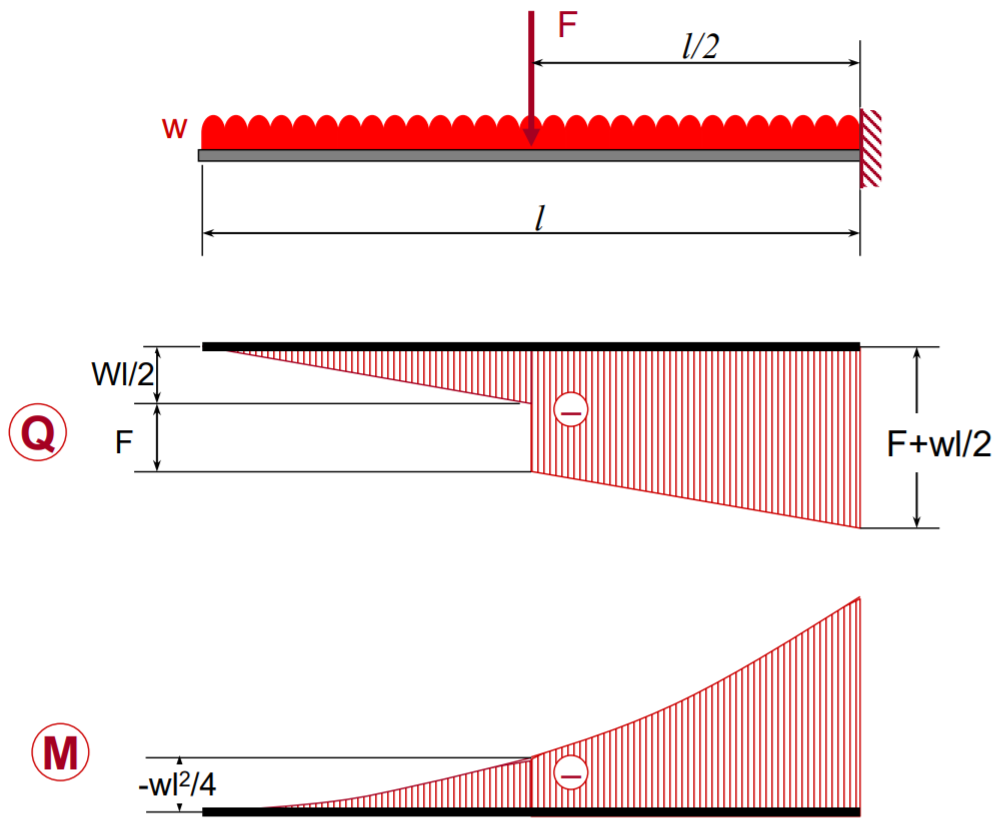
\includegraphics[width = 0.8 \textwidth]{../img/diagramofinternalforces.PNG}
\end{figure}
\end{document}